\documentclass[10pt]{article}
\usepackage{icmlko}

\icmlmeta{IP 파운데이션 월드모델}{123}{주최자 주장은 신호가 아니었다}{라벨 350건 중 75건만 쓰는 이유를 재니 --- 주최자 주장 98건만으로는 $\rho$가 $-$0.05다. 발굴은 막혔고 자연 축적은 스물한 해다}

\begin{document}

\twocolumn[
\icmlheader

\begin{abstract}
노트 122가 눈금 이야기를 닫으며 물음을 하나로 좁혔다 --- \textbf{팝업이 낮은
것이 아니라 구간이 넓다.} 그러면 답도 하나다: \textbf{몇 건을 모으면 무엇을
판정할 수 있나.} 팝업을 $n$ 건으로 줄여 가며 짝지은 차이의 구간 반폭을 재고
$n^{b}$ 를 맞췄다 --- \textbf{반폭 $=2.28\,n^{-0.88}$}. 이론값 $-$0.5보다
가파르다. 목표별 필요 표본은 137($\pm$0.030) · 217($\pm$0.020) ·
\textbf{476}($\pm$0.010) · 1,046($\pm$0.005)이고, 지금 연 18.8건이 쌓이므로
\textbf{$+$0.01짜리를 가르려면 스물한 해}가 걸린다. 그래서 발굴을 봤다.
관문을 폭포로 세니 \textbf{레코드 376건, 라벨 있는 것 350건, 실제로 쓰는 것
75건}이다. 최대 병목은 계수 방법 관문이고 \textbf{주최자 주장 247건}이 여기서
빠진다. 풀면 173건이 되니 구간이 확 좁아질 터였다. \textbf{풀어 봤다. 성적이
무너진다} --- $\rho$가 $+$0.4601에서 \textbf{$+$0.0352}로 간다. 주최자 주장만
따로 재면 \textbf{$-$0.0539}(n=98)다. \textbf{주최자 주장 방문자 수에는
예측 가능한 신호가 없다.} 실측 발자국을 $\rho{=}0.46$ 으로 맞히는 축들이
주최자 주장은 $\rho\approx0$ 으로 맞힌다. \textbf{그러므로 발굴은 막혔다} ---
있는 라벨의 79\%가 쓸 수 없는 라벨이다. 남은 길은 하나다: \textbf{앞으로 여는
팝업에 실측 계수를 붙이는 것.} 연 18.8건이 연 40건이 되면 스물한 해가 열 해가
되고, 그것이 이 프로젝트에서 가장 값싼 지렛대다 --- 축을 스물세 개 긁어 채택
0이었는데, 실측 계수 하나가 그보다 크다.
\end{abstract}
]

\begin{figure*}[t]
\centering
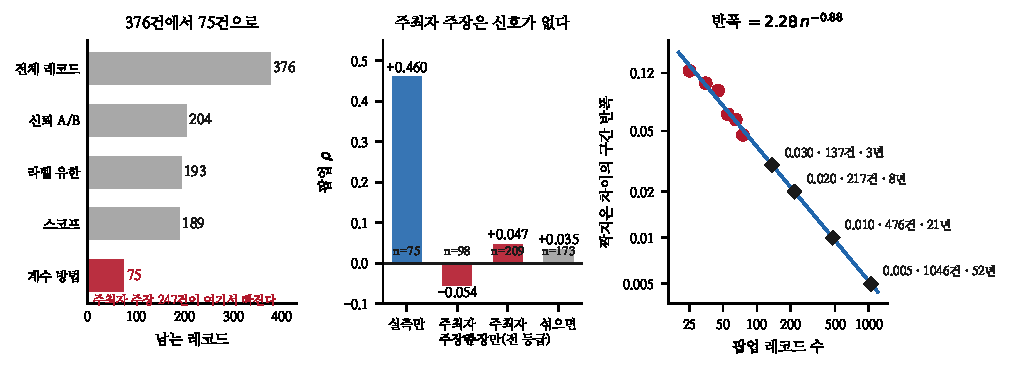
\includegraphics[width=\textwidth]{figs/pn.pdf}
\caption{왼쪽 --- 376건에서 75건으로. 가운데 --- 주최자 주장은 신호가 없다.
오른쪽 --- 반폭 $=2.28\,n^{-0.88}$.}
\end{figure*}

\section{구간은 이렇게 좁아진다}

\begin{table}[t]
\centering\tsize
\caption{팝업을 $n$ 건으로 줄이며 잰 짝지은 차이(공통 축 다섯 $-$ 셋)의
구간 반폭.}
\begin{tabular}{rrr}
\toprule
$n$ & $\Delta$ & 반폭 \\
\midrule
25 & $+$0.0175 & 0.1238 \\
35 & $+$0.0213 & 0.1028 \\
45 & $+$0.0136 & 0.0919 \\
55 & $+$0.0176 & 0.0643 \\
65 & $+$0.0101 & 0.0593 \\
75 & $+$0.0120 & 0.0471 \\
\midrule
\multicolumn{3}{l}{반폭 $=2.28\,n^{-0.88}$ \quad(이론값 $-$0.5)} \\
\bottomrule
\end{tabular}
\end{table}

\claimx{구간이 $n^{-0.88}$ 로 좁아진다 --- \textbf{$\sqrt{n}$ 보다 빠르다.}
표본이 적을 때는 팝업의 인자 공간 자체가 흔들려 잡음이 더해지기 때문으로
보인다. 모으는 값이 이론보다 크다는 뜻이다.}{여섯 점에 직선을 맞췄고 표본
뽑기가 셋뿐이다. 그리고 $n$ 을 줄이면 표본이 달라지므로 순수한 크기 효과가
아니다.}

\begin{table}[t]
\centering\tsize
\caption{목표별 필요 표본. 지금 75건, 연 18.8건.}
\begin{tabular}{rrrl}
\toprule
반폭 & $n$ & 남은 해 & 무엇을 가르나 \\
\midrule
0.030 & 137 & 3 & 지금보다 조금 낫다 \\
0.020 & 217 & 8 & $+$0.02 짜리 \\
\textbf{0.010} & \textbf{476} & \textbf{21} & \textbf{$+$0.01 짜리(대부분)} \\
0.005 & 1,046 & 52 & 노트 72의 문턱 \\
\bottomrule
\end{tabular}
\end{table}

노트 92가 설계 판정에 510건이 필요하다고 셌는데 여기서 476건이 나온다 ---
다른 방법으로 잰 두 수가 맞는다.

\section{발굴을 봤다}

\begin{table}[t]
\centering\tsize
\caption{관문 폭포.}
\begin{tabular}{lrr}
\toprule
& 남는 것 & 여기서 빠지는 것 \\
\midrule
전체 레코드 & 376 & --- \\
신뢰 등급 A/B & 204 & 172 \\
라벨 유한 & 193 & 11 \\
스코프 검증 & 189 & 4 \\
\textbf{계수 방법} & \textbf{75} & \textbf{114} \\
\midrule
\multicolumn{3}{l}{라벨이 있는 것 350건 · 실제로 쓰는 것 75건} \\
\multicolumn{3}{l}{계수 방법: 주최자 주장 \textbf{247} · 입장 54 · 참여 37} \\
\bottomrule
\end{tabular}
\end{table}

\textbf{주최자 주장이 247건이다.} 이것만 풀어도 173건이 되고 구간이 절반으로
준다. 풀어 봤다.

\section{풀었더니 무너졌다}

\begin{table}[t]
\centering\tsize
\caption{계수 방법 관문을 풀면.}
\begin{tabular}{lrr}
\toprule
& $n$ & 팝업 $\rho$ \\
\midrule
\textbf{현행(입장 · 참여)} & 75 & \textbf{$+$0.4601} \\
$+$주최자 주장 & 173 & \textbf{$+$0.0352} \\
$+$등급 C까지 & 264 & $-$0.0006 \\
전부 & 333 & $+$0.0341 \\
\midrule
\textbf{주최자 주장만} & 98 & \textbf{$-$0.0539} \\
주최자 주장만 · 등급 전부 & 209 & $+$0.0470 \\
\bottomrule
\end{tabular}
\end{table}

\claimx{\textbf{주최자 주장 방문자 수에는 예측 가능한 신호가 없다.} 실측
발자국을 $\rho{=}+$0.46 으로 맞히는 축들이 주최자 주장은 $-$0.05 로 맞힌다.
섞으면 $+$0.035 로 무너진다.}{주최자 주장 레코드가 다른 종류의 팝업일 수도
있다(작은 행사 · 오래된 것). 축이 아니라 표본이 다른 것일 가능성을 안 갈랐다.}

\begin{quote}\fontsize{9.5}{11.5}\selectfont
\textbf{관문은 지나치게 엄격한 것이 아니었다.} 그것이 모형을 살려 두는
유일한 것이었다. 그리고 이것은 사업에도 쓰는 말이다 --- \textbf{주최자가
발표하는 방문자 수로 성과를 견주면 안 된다.} 같은 기획 정보로 실측은
맞히는데 주장은 못 맞힌다.
\end{quote}

\section{그러면 남는 길은 하나다}

\begin{table}[t]
\centering\tsize
\caption{세 가지 길.}
\begin{tabular}{lll}
\toprule
길 & 얻는 것 & 판정 \\
\midrule
발굴 & 라벨 275건 & \textbf{막혔다}(신호 없음) \\
자연 축적 & 연 18.8건 & 21년 \\
\textbf{실측 계수} & \textbf{연 40건?} & \textbf{10년} \\
\bottomrule
\end{tabular}
\end{table}

\claimx{\textbf{앞으로 여는 팝업에 실측 계수를 붙이는 것이 이 프로젝트에서
가장 값싼 지렛대다.} 축을 스물세 개 긁어 채택 0이었는데(노트 116 · 117 · 118),
실측 계수 하나를 늘리는 것이 그보다 크다. 연 18.8건이 연 40건이 되면 스물한
해가 열 해가 된다.}{``연 40건''은 목표이지 측정이 아니다. 지금 주최자 주장이
연 70건쯤 쌓이므로 그중 절반에 계수기를 붙이면 되는 수치이긴 하다.}

\begin{table}[t]
\centering\tsize
\caption{무엇을 붙이나. 이미 인정되는 두 계수.}
\begin{tabular}{ll}
\toprule
\texttt{entry} & 입장 카운터 · 게이트 · 예약 체크인 \\
\texttt{participation} & 체험 참여 로그 · POS 영수증 수 \\
\bottomrule
\end{tabular}
\end{table}

\section{한계}

\begin{itemize}[leftmargin=1.1em,itemsep=0.15em]
\item \textbf{채택할 것이 없다.} 이 노트는 설정을 안 바꾼다.
\item 주최자 주장이 신호가 없는 것인지 \emph{그 표본}이 다른 것인지 안 갈랐다.
\item 반폭 곡선이 여섯 점이고 표본 뽑기가 셋이다. 21년은 눈금이지 예측이
      아니다.
\item 연 18.8건은 2023--2026의 평균인데 2025년만 40건이라 최근 속도는 더
      빠를 수 있다.
\item 노트 120의 정직한 눈금으로 도구 문서를 고치는 일은 아직 안 했다.
\end{itemize}

\section{다음}

\begin{enumerate}[leftmargin=1.3em,itemsep=0.15em]
\item \textbf{주최자 주장을 한 번 더 판다} --- 신호가 없는 것인지 표본이
      다른 것인지. 같은 IP · 같은 자리에서 주장과 실측이 둘 다 있는 짝을
      찾으면 바로 갈린다.
\item \textbf{도구 문서를 고친다}(노트 122가 남긴 것) --- \texttt{state/score.py}
      의 자기 검사와 노트 91의 순위표를 정직한 눈금으로.
\item \textbf{계수기 붙이기 지침} --- \texttt{entry} · \texttt{participation}
      으로 인정되는 계수의 최소 요건을 한 장으로 적는다.
\item 남은 다섯 도메인의 정직한 라벨.
\end{enumerate}

\vspace{0.6em}
\hrule height 0.3pt
\vspace{0.5em}
{\footnotesize
\textbf{참고문헌}\\[0.3em]
Varoquaux, G. (2018). Cross-validation failure: small sample sizes lead to large
error bars. \emph{NeuroImage}, 180, 68--77.\\[0.15em]
Efron, B., Tibshirani, R. J. (1993). \emph{An Introduction to the Bootstrap}.
Chapman \& Hall.\\[0.15em]
Lord, F. M., Novick, M. R. (1968). \emph{Statistical Theories of Mental Test
Scores}. Addison-Wesley.\\[0.15em]
Halevy, A., Norvig, P., Pereira, F. (2009). The unreasonable effectiveness of
data. \emph{IEEE Intelligent Systems}, 24(2), 8--12.\\[0.15em]
Ben-David, S. et al. (2010). A theory of learning from different domains.
\emph{Machine Learning}, 79(1--2), 151--175.
}

\end{document}
